


\documentclass[aspectratio=169,11pt]{beamer}

% -------------------------------------------------
% NASA SPACE APPS CHALLENGE — 5-SLIDE PRESENTATION
% Compile with pdfLaTeX on Overleaf.
% -------------------------------------------------

\usetheme{default}
\usepackage[T1]{fontenc}
\usepackage{lmodern}
\usepackage{graphicx}
\usepackage{booktabs}
\usepackage{amsmath}
\usepackage{tikz}
\usetikzlibrary{calc,positioning,shadows.blur}

% Space palette
\definecolor{spacebg}{HTML}{071426}
\definecolor{spacepanel}{HTML}{10243D}
\definecolor{nebula}{HTML}{173B63}
\definecolor{starlight}{HTML}{F2F6FC}
\definecolor{muted}{HTML}{B8C7D9}
\definecolor{nasaorange}{HTML}{FF8A3D}
\definecolor{orbitblue}{HTML}{55B7E8}

% Beamer colors and layout
\setbeamercolor{background canvas}{bg=spacebg}
\setbeamercolor{normal text}{fg=starlight}
\setbeamercolor{frametitle}{fg=starlight,bg=spacebg}
\setbeamercolor{title}{fg=starlight}
\setbeamercolor{subtitle}{fg=muted}
\setbeamercolor{structure}{fg=orbitblue}
\setbeamercolor{itemize item}{fg=nasaorange}
\setbeamercolor{itemize subitem}{fg=orbitblue}
\setbeamercolor{block title}{fg=white,bg=nebula}
\setbeamercolor{block body}{fg=starlight,bg=spacepanel}
\setbeamercolor{alerted text}{fg=nasaorange}
\setbeamertemplate{navigation symbols}{}
\setbeamertemplate{itemize item}{\raisebox{0.15ex}{\tiny$\blacktriangleright$}}
\setbeamertemplate{itemize subitem}{\tiny$\bullet$}
\setbeamertemplate{headline}{}
\setbeamertemplate{footline}{
  \leavevmode
  \hbox{
    \begin{beamercolorbox}[wd=.82\paperwidth,ht=2.7ex,dp=1.1ex,leftskip=1em]{author in head/foot}
      \color{muted}\scriptsize 2026 NASA SPACE APPS CHALLENGE
    \end{beamercolorbox}
    \begin{beamercolorbox}[wd=.18\paperwidth,ht=2.7ex,dp=1.1ex,rightskip=1em plus 1fil]{date in head/foot}
      \color{muted}\scriptsize \insertframenumber/\inserttotalframenumber
    \end{beamercolorbox}
  }
}
\setbeamertemplate{frametitle}{
  \vspace{0.45cm}
  \insertframetitle
  \par\vspace{0.12cm}
  {\color{orbitblue}\rule{0.14\paperwidth}{1.2pt}}
}

% Decorative star field
\newcommand{\starfield}{
  \begin{tikzpicture}[remember picture,overlay]
    \foreach \x/\y/\r in {
      0.7/0.8/0.45,1.8/2.9/0.35,3.2/1.2/0.55,4.5/3.4/0.35,
      5.9/0.55/0.4,7.1/2.6/0.45,8.4/0.9/0.35,9.7/3.2/0.5,
      11.1/1.5/0.4,12.4/2.8/0.35,2.5/5.8/0.4,6.4/5.5/0.35,
      10.8/5.9/0.45,12.7/4.8/0.35
    }{
      \fill[white,opacity=0.45] ([xshift=\x cm,yshift=\y cm]current page.south west)
        circle[radius=\r pt];
    }
    \draw[orbitblue,opacity=0.12,line width=0.6pt]
      ([xshift=9.7cm,yshift=0.25cm]current page.south west)
      ellipse[x radius=3.0cm,y radius=0.8cm,rotate=18];
  \end{tikzpicture}
}
\newcommand{\eyebrow}[1]{%
  {\color{muted}\scriptsize\MakeUppercase{#1}}\par\vspace{0.18cm}
}

\begin{document}

% -------------------------------------------------
% SLIDE 1 — INTRODUCTION / TITLE
% -------------------------------------------------
{
\setbeamertemplate{footline}{}
\begin{frame}[plain]
  \starfield
  \begin{tikzpicture}[remember picture,overlay]
    \shade[ball color=orbitblue!75!black]
      ([xshift=-3cm,yshift=-5.0cm]current page.north east) circle (1.45cm);
    \draw[orbitblue!80,opacity=.65,line width=1pt]
      ([xshift=-3cm,yshift=-5.0cm]current page.north east)
      ellipse[x radius=2.1cm,y radius=.48cm,rotate=-18];
    % \fill[nasaorange] ([xshift=-3.3cm,yshift=-4.8cm]current page.north east)
    %   circle (0.08cm);
  \end{tikzpicture}

  \vspace{0.45cm}
  {\color{nasaorange}\scriptsize 2026 NASA SPACE APPS CHALLENGE}\par
  \vspace{0.35cm}
  {\fontsize{27}{32}\selectfont\bfseries
    Space Mission Design Game Challenge\par}
  \vspace{0.55cm}
  {\large\color{muted}A game for designing and exploring space missions\par}
  \vspace{0.5cm}
  {\normalsize\bfseries\color{orbitblue}Team: Curious Explorers\par}
  \vspace{0.22cm}
  {\normalsize Abdelaziz Nematallah \quad Anna Dembowski \quad Asem Shrafelden\par}
  \vspace{0.18cm}
  {\small\color{muted}BTU Cottbus-Senftenberg\par}
  \vfill
  {\scriptsize\color{muted}November 15, 2026}
\end{frame}
}

% -------------------------------------------------
% SLIDE 2 — MOTIVATION
% -------------------------------------------------
\begin{frame}{Challenge and Approach}
  \vspace{0.1cm}
  {\large An interactive game to design, manage and simulate a complete space mission.}\par
  \vspace{0.38cm}
  \begin{center}
  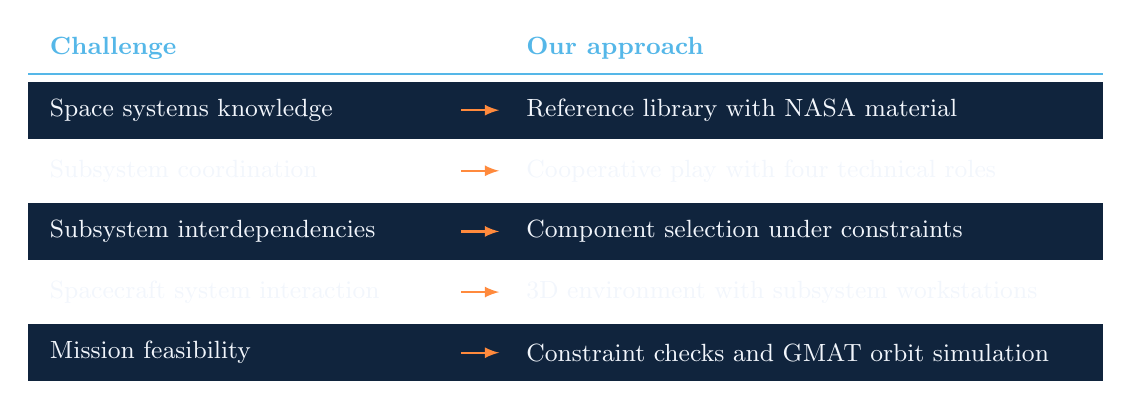
\begin{tikzpicture}[
    heading/.style={anchor=west,text=orbitblue,font=\small\bfseries},
    challenge/.style={anchor=west,text=starlight,font=\small},
    response/.style={anchor=west,text=starlight,font=\small},
    link/.style={-latex,draw=nasaorange,line width=.8pt}]
    \node[heading] at (.15,.1) {Challenge};
    \node[heading] at (6.2,.1) {Our approach};
    \draw[orbitblue,line width=.5pt] (0,-.23)--(13.65,-.23);
    \foreach \y in {-.69,-2.23,-3.77} {
      \fill[spacepanel] (0,\y+.36) rectangle (13.65,\y-.36);
    }
    \node[challenge] at (.15,-.69) {Space systems knowledge};
    \node[response] at (6.2,-.69) {Reference library with NASA material};
    \node[challenge] at (.15,-1.46) {Subsystem coordination};
    \node[response] at (6.2,-1.46) {Cooperative play with four technical roles};
    \node[challenge] at (.15,-2.23) {Subsystem interdependencies};
    \node[response] at (6.2,-2.23) {Component selection under constraints};
    \node[challenge] at (.15,-3.00) {Spacecraft system interaction};
    \node[response] at (6.2,-3.00) {3D environment with subsystem workstations};
    \node[challenge] at (.15,-3.77) {Mission feasibility};
    \node[response] at (6.2,-3.77) {Constraint checks and GMAT orbit simulation};
    \foreach \y in {-.69,-1.46,-2.23,-3.00,-3.77} {
      \draw[link] (5.5,\y)--(5.98,\y);
    }
  \end{tikzpicture}
  \end{center}
\end{frame}

% -------------------------------------------------
% SLIDE 3 — GAME WORKFLOW
% Based on the supplied game's assembly, design and operations modules.
% -------------------------------------------------
\begin{frame}{Game Design}
  \vspace{0.15cm}
  {\color{muted}Up To Four Players Share Four Distinct Technical Roles.}\par
  \vspace{0.6cm}
  \begin{center}
  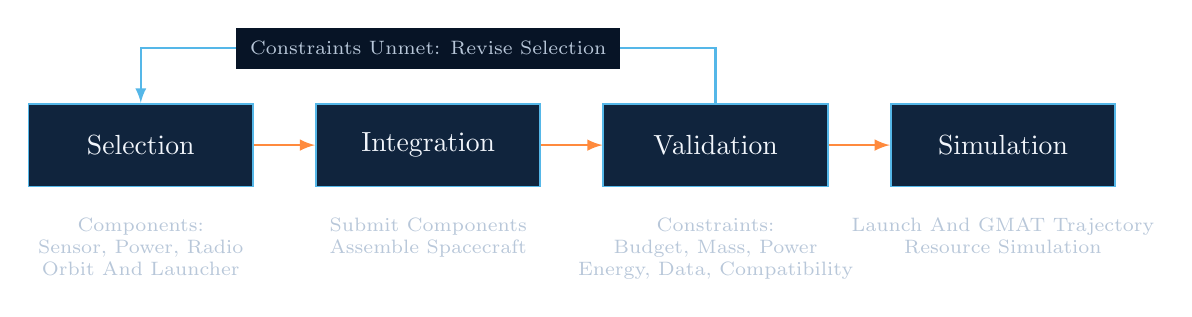
\begin{tikzpicture}[
    stage/.style={draw=orbitblue,line width=.65pt,fill=spacepanel,
      minimum width=2.85cm,minimum height=1.05cm,text=starlight,
      font=\normalsize,align=center},
    detail/.style={text=muted,font=\scriptsize,align=center},
    flow/.style={-latex,draw=nasaorange,line width=.9pt}]
    \node[stage] (design) at (0,0) {Selection};
    \node[stage] (integration) at (3.65,0) {Integration};
    \node[stage] (validation) at (7.3,0) {Validation};
    \node[stage] (operate) at (10.95,0) {Simulation};
    \draw[flow] (design)--(integration);
    \draw[flow] (integration)--(validation);
    \draw[flow] (validation)--(operate);
    \node[detail,anchor=north] at (0,-.8) {Components:\\Sensor, Power, Radio\\Orbit And Launcher};
    \node[detail,anchor=north] at (3.65,-.8) {Submit Components\\Assemble Spacecraft};
    \node[detail,anchor=north] at (7.3,-.8) {Constraints:\\Budget, Mass, Power\\Energy, Data, Compatibility};
    \node[detail,anchor=north] at (10.95,-.8) {Launch And GMAT Trajectory\\Resource Simulation};
    \draw[-latex,draw=orbitblue,line width=.8pt]
      (validation.north) -- ++(0,.70) -| (design.north);
    \node[detail,fill=spacebg,inner sep=5pt] at (3.65,1.23) {Constraints Unmet: Revise Selection};
  \end{tikzpicture}
  \end{center}
  \vspace{0.45cm}
  {\small Players Move Between Subsystem Workshops And Assemble One Shared Spacecraft.}
\end{frame}

% -------------------------------------------------
% SLIDE 4 — LIVE DEMO
% -------------------------------------------------
{
\setbeamertemplate{footline}{}
\begin{frame}[plain]
  \starfield
  \begin{tikzpicture}[remember picture,overlay]
    \shade[ball color=orbitblue!70!black]
      ([xshift=-2.0cm,yshift=-2.1cm]current page.north east) circle (1.0cm);
    \draw[nasaorange,opacity=.8,line width=1pt]
      ([xshift=-2.0cm,yshift=-2.1cm]current page.north east)
      ellipse[x radius=1.55cm,y radius=.38cm,rotate=-20];
  \end{tikzpicture}
  \vfill
  \begin{center}
    {\color{nasaorange}\scriptsize SYSTEMS CHECK: READY}\par
    \vspace{0.35cm}
    {\fontsize{36}{42}\selectfont\bfseries LIVE DEMO}\par
    \vspace{0.35cm}
    {\Large\color{muted}See the mission design game in action}\par
    \vspace{0.8cm}
    
\begin{tikzpicture}
      \draw[orbitblue,line width=1.2pt,rounded corners=4pt] (0,0) rectangle (4.2,1.0);
      \node[text=starlight,execute at begin node={\hyphenpenalty=10000\exhyphenpenalty=10000},font=\large\bfseries] at (2.1,.5) {DEMO};
      \fill[nasaorange] (-.25,.5) circle (2pt);
      \fill[nasaorange] (4.45,.5) circle (2pt);
    \end{tikzpicture}
  \end{center}
  \vfill
\end{frame}
}

% -------------------------------------------------
% SLIDE 5 — IMPROVEMENTS
% -------------------------------------------------
\begin{frame}{Planned Extensions}
  \setbeamerfont{block title}{size=\normalsize}
  \small
  % \starfield
  % \eyebrow{Next steps for the project}
  \begin{columns}[T,onlytextwidth]
    \column{0.64\textwidth}
      \begin{block}{Mission and spacecraft options}
        \small
        \begin{itemize}
          \setlength{\itemsep}{1pt}
          \setlength{\parskip}{0pt}
          \item Mission-specific objectives and budgets.
          \item Additional sensors, power systems and radios.
          \item Selectable orbit altitude and inclination.
        \end{itemize}
      \end{block}
      \begin{block}{Worked engineering examples}
        \small Add library examples for power budgets, data storage and ground-station contacts.
      \end{block}

    \column{0.29\textwidth}
      \centering
      
\begin{tikzpicture}
        \shade[ball color=orbitblue!65!black] (0,0) circle (.72cm);
        \draw[orbitblue,line width=1pt] (0,0) ellipse (1.15cm and .38cm);
        \draw[nasaorange,line width=1pt] (0,0) ellipse (1.55cm and .55cm);
        \fill[starlight] (1.5,.12) circle (2.4pt);
        \fill[nasaorange] (-1.05,.31) circle (2.4pt);
        \node[text=starlight,execute at begin node={\hyphenpenalty=10000\exhyphenpenalty=10000},font=\bfseries] at (0,-1.25) {NEXT};
        \node[text=muted,font=\scriptsize] at (0,-1.58) {MISSION UPDATES};
      \end{tikzpicture}
  \end{columns}
  % \vfill
  % {\color{orbitblue}\bfseries Thank you!}
  % \hfill
  % {\scriptsize\color{muted}Questions?}
\end{frame}

\end{document}





